\chapter{Methods}

\section{Simulation of capacitance} \label{sec.analysecurrent}
The dependency of $C_0$ has to be simulated numerically for the high-voltage setup as well as for the low-voltage setup. 
\begin{figure}[htbp]
	\centering
	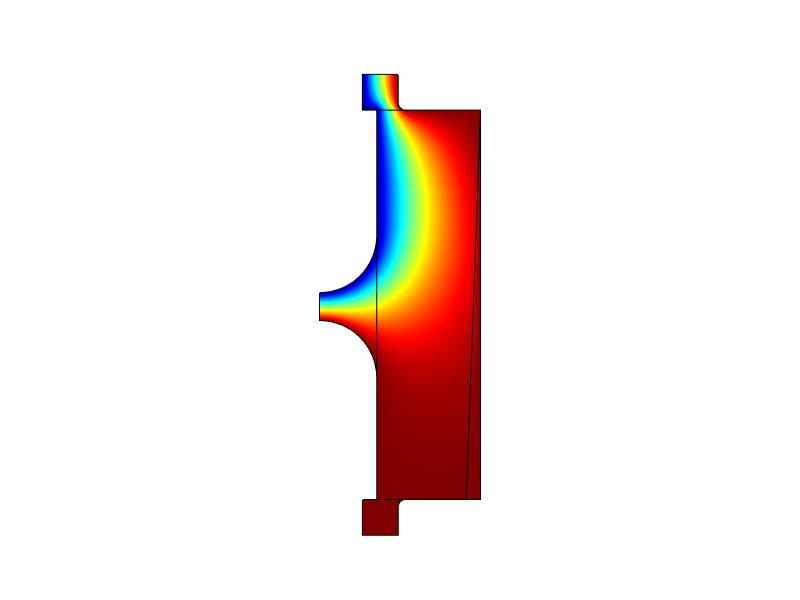
\includegraphics{figures/COMSOL_Beispielbild.jpg}		
	\caption[Kurze Abbildungsbeschreibung]{Field simulation of the low-voltage test cell (0.5 mm electrode distance)} \ref{sec.analysecurrent}
	\label{fig.waveforms}
\end{figure}
 

\section{Signal analysis of the Debye model}

In order to emulate different dielectrica with their own respective dielectric loss tangent, different combinations of circuit elements were used. Each different circuit accounts for another loss tangent with respect to frequency. With the objective to assess the performance of the current transformer, reasonably high values for the $tan\left(\delta\right)$ were assumed (i.e. 0.05 to 0.2) since a lower loss tangent would require a higher resolution on the part of the current measurement.


\begin{figure}[htbp]
	\centering
	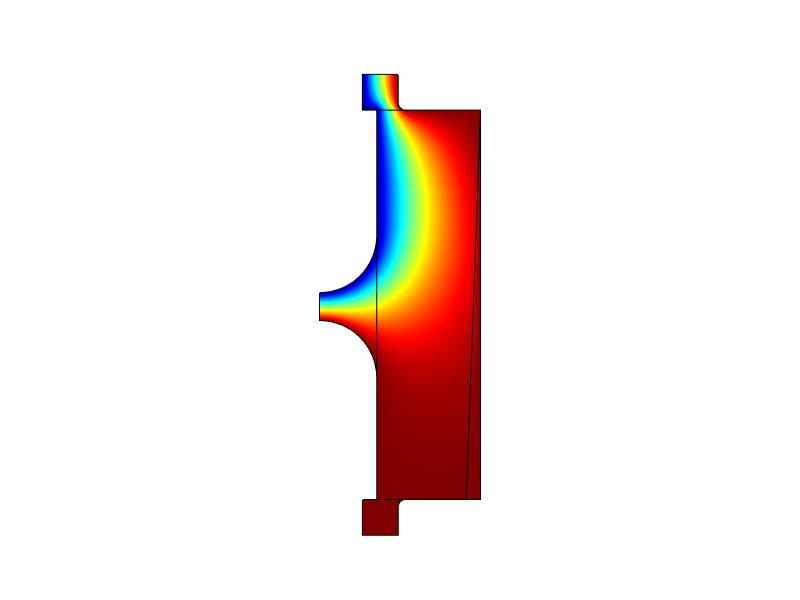
\includegraphics{figures/COMSOL_Beispielbild.jpg}		
	\caption[Kurze Abbildungsbeschreibung]{Electron drift currents in Ar at 30 Td and in CO$_2$ at 65 Td, the latter was divided by 10 and shifted by 0.2 $\mu$s. Dotted lines are averages of measured waveforms, solid lines are fits of Eq. XX. $T$ marks the electron transit time, and the markers $T_1$ to $T_3$ are explained in section.} \ref{sec.analysecurrent}
	\label{fig.waveforms}
\end{figure}

\section{Measurement of the \epsilon and the tan($\delta$) for the Debye model}
The aim is to have a current flwoing though the Debye model in the low-voltage setup that is oft the same order as a current in the high voltage-setup. In order to have a comparable current for a voltage that is $1/1000$ of the high-voltage setup a capacitance $C_0$ for the Debye is selected 1000 times higher than the Capacitance of the samples. As the sample has a capacitance of 3.44 pF its equivalent $C_0$ in the debye-model is 3.3 nF. In order to get a tan($\delta$) of !!! $R_i$ is chosen as and $C_i$ is chosen as .

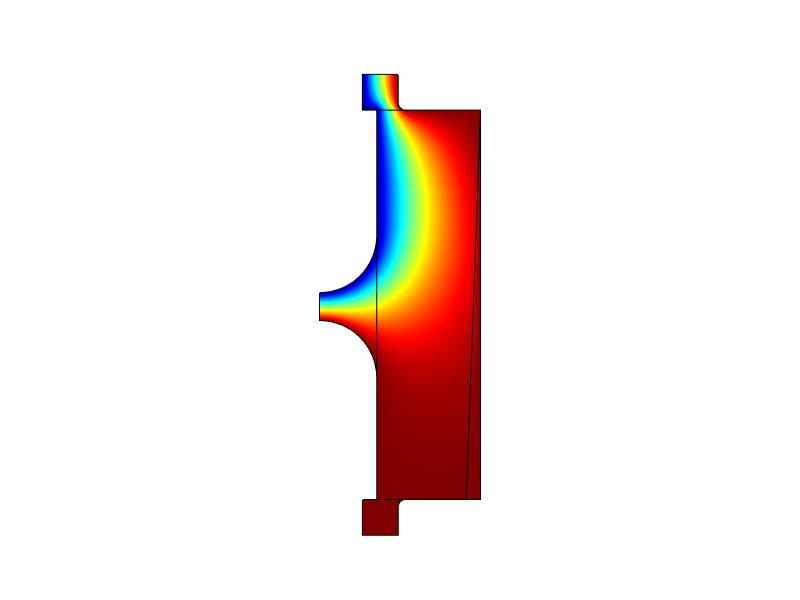
\includegraphics{figures/COMSOL_Beispielbild.jpg}		
